\section{Оборудование и инструментальные погрешности}

\begin{wrapfigure}{r}{0.25\textwidth}
    \centering
    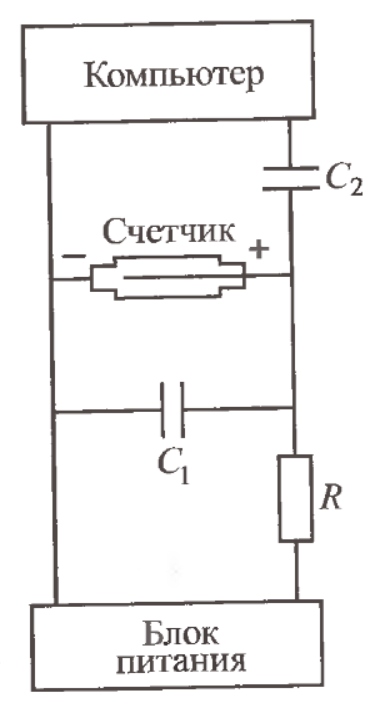
\includegraphics[width=0.2\textwidth]{img/counter.png}
\end{wrapfigure}

Для обнаружения и измерения интенсивности космических лучей используется
счётчик Гейгера--Мюллера. Он представляет собой тонкостенный металический цилиндр
с проводящей нитью в центре и газом в камере. К электродам приложено напряжение.
При прохождении частицы через счётчик возникает лавина электронов, которая
приводит к появлению тока.

Схема включения счётчика приведена на рисунке. Через сопротивление $R$
на счётчик от блока питания подаётся сопротивление. В исходном состоянии
электроды и конденсатор $C_1$ заряжены до $400\,\text{В}$. Конденсатор
$C_2$ не пропускает постоянное напряжение источника питания в интерфейсные
схемы компьютера. При возникновении тока через источник заряд на счётчике и $C_1$
обеспечивает развитие электронной лавины на короткое время. При разряде энергия
поступает от от заряженного конденсатора $C_1$. После лавины схема приходит
в исходное состояние за время порядка нескольких $RC_1$. При этом через $C_2$
на компьютер передаётся короткий импульс. Значительную часть регистрируемых частиц
составляет естественный радиоактивный фон.

Ошибки в измерениях счётчика малы по сравнению с изменением фона. Погрешности
измерений определяются в основном временем, в течении которого восстанавливаются нормальные
условия в схеме. 
